\newpage
\thispagestyle{empty}
\mbox{}

\chapter{Parrafor en sucio}
\label{ch:chapter6}


En donde, $\sigma$ es la desviación típica aportando información sobre la variación de la concentración de las sustancias y $\mu$ la media que representa el punto de máxima radiación de la fuente. Un aspecto relevante es que si el centro de la formación se encuentra lo suficientemente cerca de la fuente el argumento de la exponencial tenderá a 0 conllevando a que en torno a dicho punto se tenga la máxima concentración de sustancias.

\begin{figure}[htb]
\centering
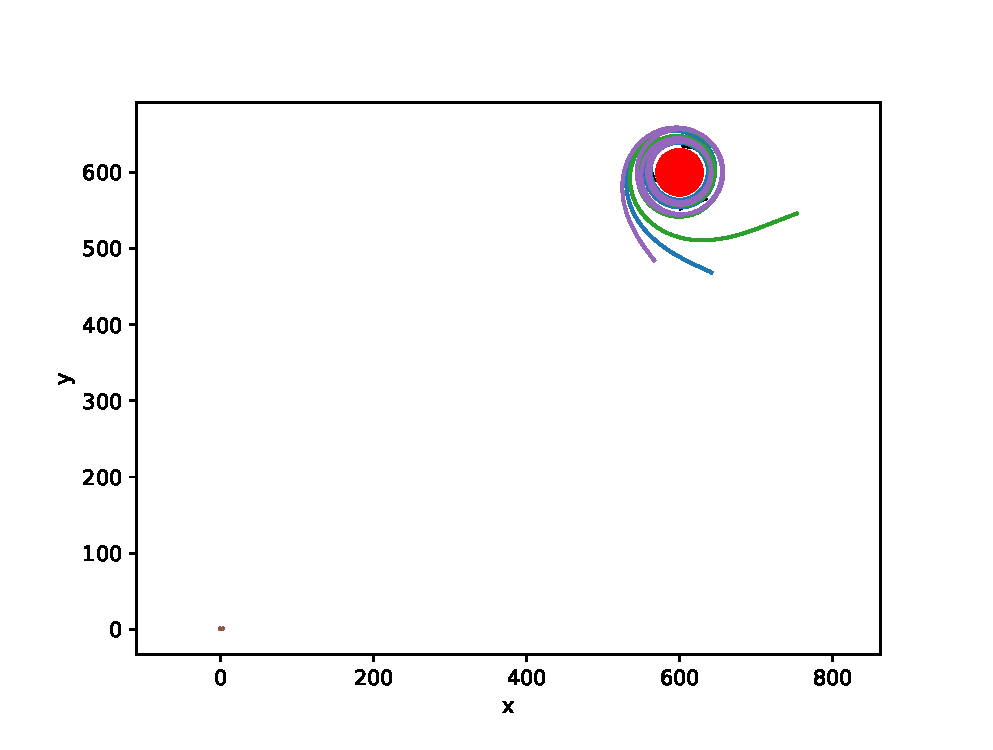
\includegraphics[width=0.85\textwidth]{figures/Coordinacion/Objetivo_Final.eps}
\caption{Vehículos dispuestos en torno a la formación. El punto rojo representa el circulo al que quieren converger y las diferentes líneas que giran en torno a dicho punto son cada una de las trayectorias de los vehículos.} \label{Ejemplo_Coordinacion}
\end{figure}

\begin{figure}[H]
\centering
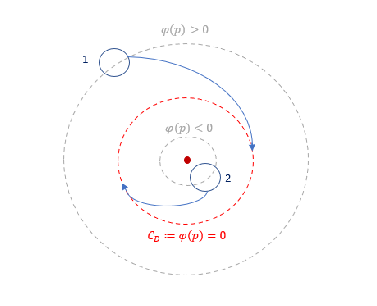
\includegraphics[width=0.60\textwidth]{figures/Pruea_Coordinacion.eps}
\caption{Ejemplo del algoritmo de control de formación} \label{Ejemplo_Coordinacion}
\end{figure}

No obstante, el algoritmo a su vez debería de estar acotado por el número de agentes que a pesar de influir en menor medida también deben de tomarse en cuenta para dicha cota.

En la realidad el avance vendrá dado por la toma de manera continúa del nivel de contaminación dado por los sensores de cada uno de los USVs, en donde, se obtendrá una dirección de avance descrita por el gradiente en cada punto. No obstante, en simulación el sistema en sí debe tener la capacidad de dirigirse hacia la zona de interés por ello es que se va a hacer uso del \textbf{algoritmo de ascenso}. Ante este algoritmo surge la hipótesis de que la función utilizada para la simulación necesariamente ha de ser cóncava para definir un punto máximo y así poder desplazarte de manera ascendente hasta dicho punto.\\

\begin{figure}[H]
\centering
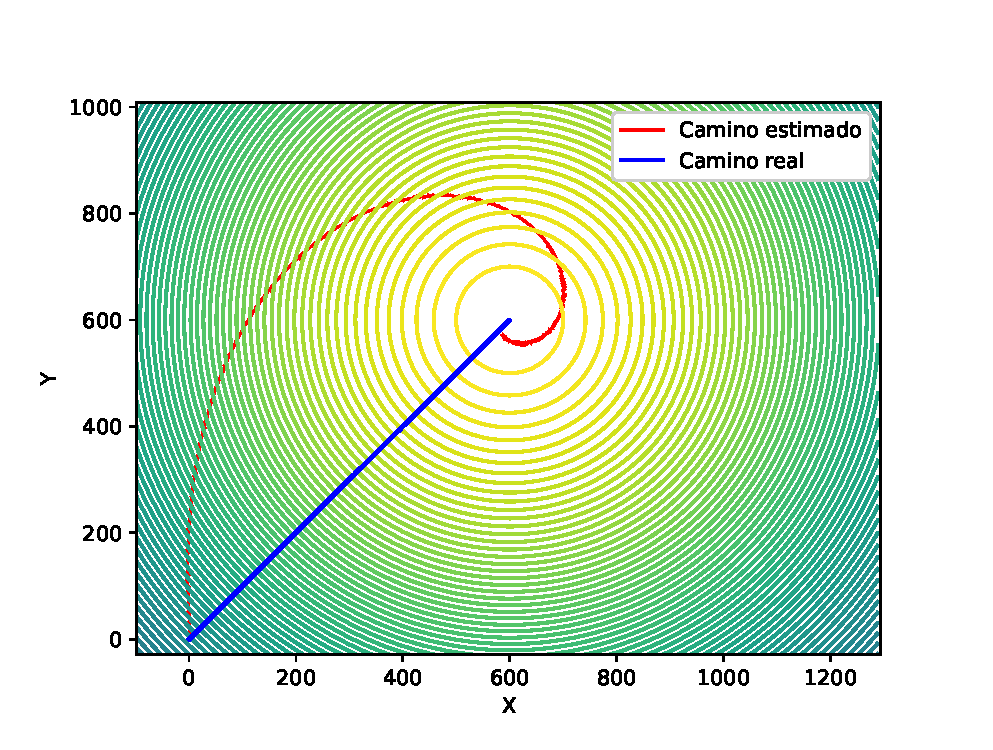
\includegraphics[width=0.70\textwidth]{figures/Caso_Inicial/Caminos.eps}
\caption{Comparativa entre el camino descrito por el gradiente real y por el gradiente estimado.} \label{Dif_Caminos}
\end{figure}

Para la obtención del gradiente, se adoptan los \textbf{algoritmos de tipo consenso} siendo estos un mecanismo que permite a maquinas coordinarse en un entorno distribuido, es decir, encuentran la solución al problema de la comunicación entre diferentes entes aislados con el objetivo de ponerse de acuerdo para realizar una tarea concreta.










La figura \ref{Curva_error} describe el error dado por la ecuación \ref{error_gradiente}. En este se ve como claramente según se va acercado el conjunto de robots al máximo, el error se va disminuyendo y a la vez que el valor del gradiente tiende a 0 traduciéndose eso en la ecuación \ref{GA} que el avance es menor. Dicha situación se puede aprovechar para evaluar bajo que condiciones el algoritmo funciona mejor, es decir, tal como se describió en la sección \ref{Objetivos_Principales}. Finalmente, es importante evaluar la relación existente entre $\Delta{\nabla{f\left(c\right)}}$ y $\hat{\nabla}{f\left(c\right)}$ con los diferentes parámetros del sistema.


Finalmente, todas las simulaciones obtenidas a lo largo de este capitulo se basaron en \cite{Git_Hector}, el cual contiene el algoritmo de coordinación original y \cite{Git_todos} contiene las modificaciones necesarias para que los tres algoritmos funcionen en conjunto.